In this section we'll present and analyze the main components in which our system is divided and we'll explain the relations between them.
\subsection{Database}
\label{subsect:Database}
			\todo{TODO ER + description}
			
\subsection{Application Server}
\label{subsect:Application Server}
			\begin{figure}[H]
				\begin{center}
					\hspace*{-60pt}
					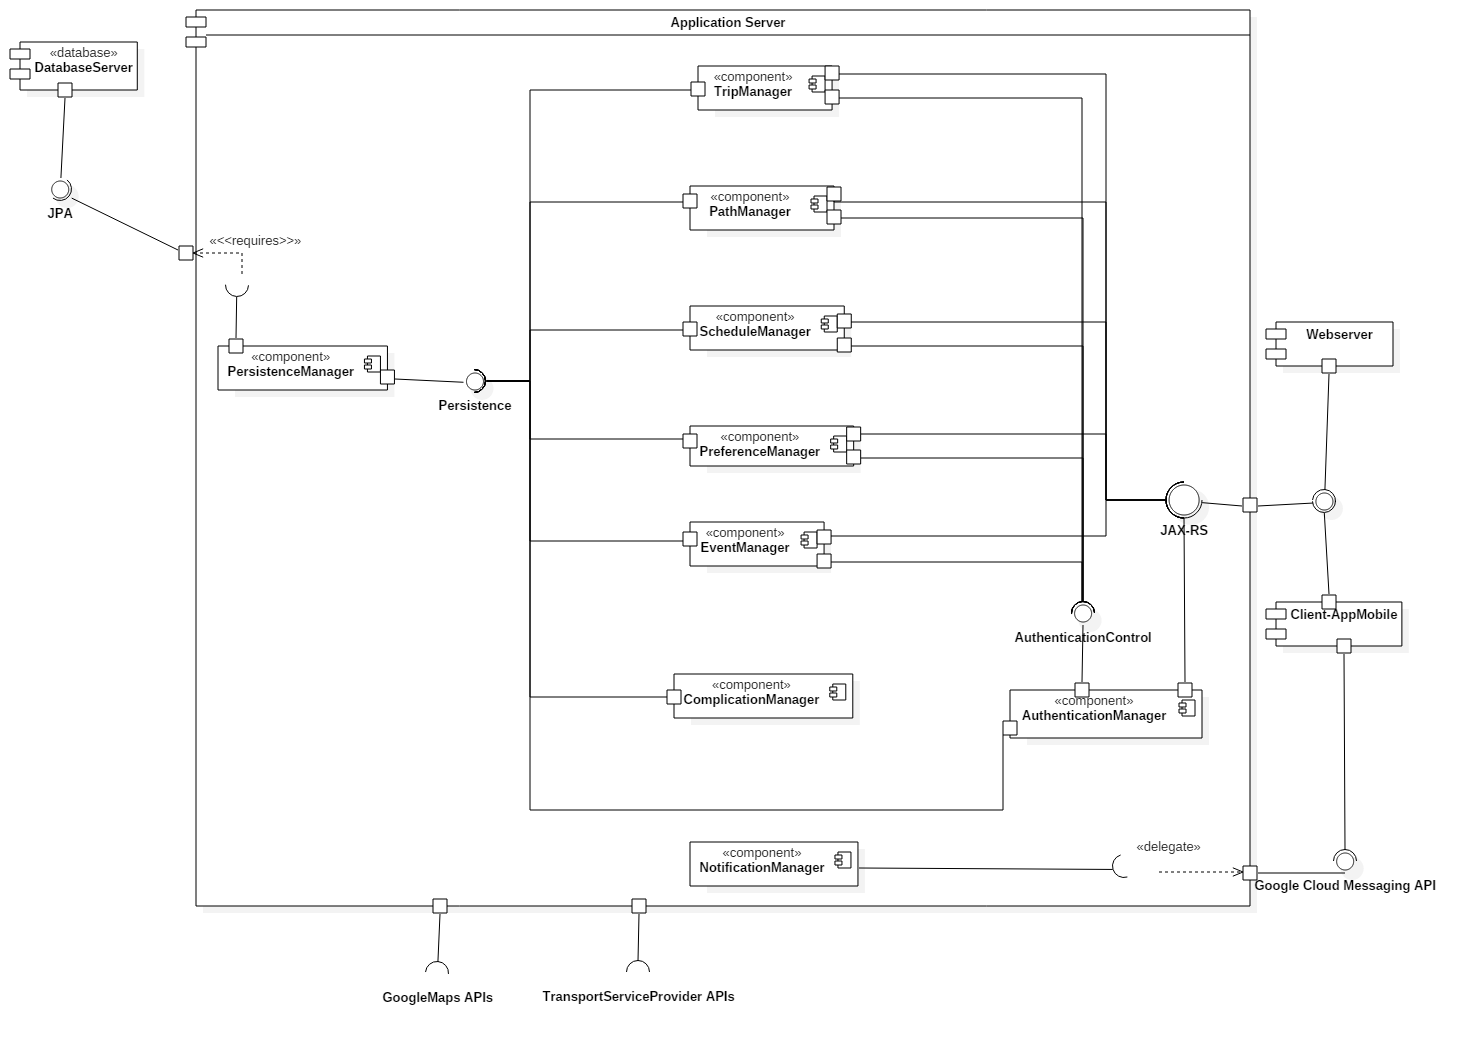
\includegraphics[scale=0.4]{ApplicationServer.png}
				\end{center}
				\caption{The components of the Application Server}
			\end{figure}
The application server must handle the whole business logic of the application, the connection with the data layer and it must expose all the needed functionalities to the users. It also has to interact with external systems. \\ \\
The main application server components are:
\begin{itemize}
	\item \textbf{AuthenticationManager:} This module will manage the user registration, the user login and it will be involved in any user request to the application server in order to check if the request comes from an authorized device.
	\item \textbf{PathManager:} This module will manage the user travels computation, after the insertion or the modification of an event or also after a specific user requests to change a selected path. It will compute the feasible paths through the invocation of Google Maps API and it will also interact with the PreferenceManager in order to obtain the information needed to guarantee that the user preferences are respected in every proposed path. 
	\item \textbf{EventManager:} This module will manage the insertion, deletion and modification of the events into the user calendar. It will interact with the ScheduleManager in order to find out if an event does overlap with others events. When an event is created it will involve the PathManager in order to provide feasible paths to reach the inserted events. It will also handle insertion, deletion and modification of the flexible breaks. \\
	If the users has inserted one or more periodic events, this module will handle their propagation in the time. 
	\item \textbf{ScheduleManager:} This module will manage the event's scheduling functionalities: it is able to check if an event overlaps with others events and to guarantee that the flexible breaks are respected. It will also check that the user's travels does not overlap with other events. When an event overlaps with another one, it will put it in a separate list of non scheduled events and it will manage the user's requests of rescheduling these events.
	\item \textbf{PreferenceManager:} This module will offer all the functionalities needed to insert, modify and delete the user's event profiles. It will also interact with the module that has to apply the event profiles in order to compute the travel paths(PathManager).
	\item \textbf{TripManager:} This module will provide the logic needed to arrange the users trips; to do so, this module will interact with external systems of Transport service providers in order to allow the user to buy public transportation tickets or to locate the nearest vehicle of a sharing system when those travel means are involved in the user's travel path.
	\item \textbf{ComplicationManager:} This module will periodically checks if the travels that are close in time are still feasible. To do so it will interact with external systems of Transport service providers to gain information about strikes, with open weather APIs to obtain information about the weather and with Google Maps APIs to obtain information about the traffic. If this module detects that a travel is no more a feasible one, it will charge the NotificationManager to warn the involved user.
	\item \textbf{NotificationManager:} This module will serve as a gateway to all the notifications to be sent, from others modules, to the user's mobile devices. To do so it will use the Google Cloud Messaging APIs in order to ensure a transparent interface with both IOS and android devices.
	\item \textbf{PersistenceManager:} This module will provide transparent access to the database functionalities from all the others modules. All system database functionalities must be developed inside this module.
\end{itemize}
\subsection{Web Server}
\label{subsect:Web Server}
	The web server layer connects the users that wants to use Travlendar+ through a web browser with the Application Server. \newline
	The main functions to be implemented in this layer are basically interfaces.
	The only logic in this layer is used to embed a map into the relative web page and to draw the paths the user must travel to reach his events. To do so the web browser will interact with Google Polylines APIs.\newline
	The presentation will be handled by the JavaServerPages component that will be implemented using JSP pages. The interaction with the Application server and with the maps API will be handled by the WebController module.

\subsection{App Mobile}
\label{subsect:App Mobile}
	The web server layer connects the users that want to use Travlendar+ through their mobile devices with the Application Server.
	To do so it uses three main modules: the GUIManager will handle all the presentation functionalities of the app, the DBManager will handle all the users data, such as events and some information about travels duration, in order to enable the user to use some of the app functionalities even when he does not have access to an Internet connection, the ApplicationController will handle the interaction with the server, using the inputs provided by the users through the GUIManager and also requesting data manipulation operations in the local app database with the information received from the server. The application controller will also handle the notifications received and it will interact with Google Polylines APIs for mobile devices in order to to draw the paths the user must travel to reach his events and provide GPS path following functionalities.
	
\begin{figure}[H]
\begin{center}
		\hspace*{-0pt}
		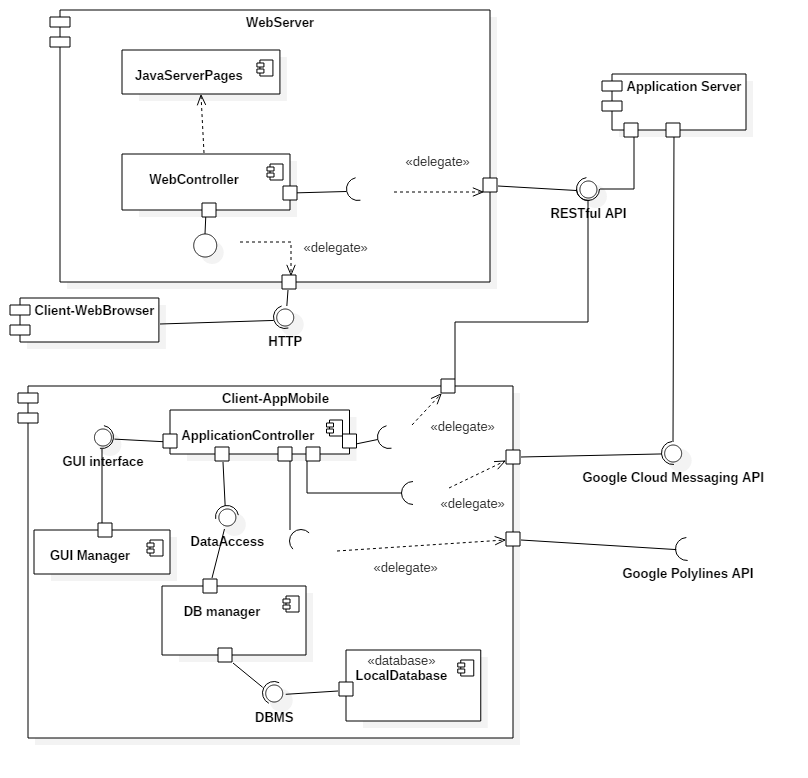
\includegraphics[scale=0.5]{Client_and_web_server.png}
\end{center}
\caption{The components of the web server, of the client app and of the client browser}
\end{figure}
\todo{TODO implementation choices in the Application server are still to be written}
Our implementation choice will be to use Java Enterprise Edition 7 (JEE)
In order to provide a mean to interface to the client and the web server the application server will use 